%%%%%%%%%%%%%%%%%%%%%%%%%%%%%%%%%%%%%%%%%%%%%%%%%%%%%%%%%%%%%%%%%%%%%%%%%%%%%%%%
%                         FORMATO DE TESIS FI UNAM                             %
%%%%%%%%%%%%%%%%%%%%%%%%%%%%%%%%%%%%%%%%%%%%%%%%%%%%%%%%%%%%%%%%%%%%%%%%%%%%%%%%
% based on Harish Bhanderi's PhD/MPhil template, then Uni Cambridge
% http://www-h.eng.cam.ac.uk/help/tpl/textprocessing/ThesisStyle/
% corrected and extended in 2007 by Jakob Suckale, then MPI-iCBG PhD programme
% and made available through OpenWetWare.org - the free biology wiki

%                     Under GNU License v3

% ADAPTADO PARA FI-UNAM:  Jesús Velázquez y Marco Ruiz

\documentclass[twoside,11pt]{Latex/Classes/PhDthesisPSnPDF}
%         PUEDEN INCLUIR EN ESTE ESPACIO LOS PAQUETES EXTRA, O BIEN, EN EL ARCHIVO "PhDthesisPSnPDF.cls" EN "./Latex/Classes/"
\usepackage{blindtext}                        % Para insertar texto dummy, de ejemplo, pues.
% Note:
% The \blindtext or \Blindtext commands throughout this template generate dummy text
% to fill the template out. These commands should all be removed when 
% writing thesis content.
% This file contains macros that can be called up from connected TeX files
% It helps to summarise repeated code, e.g. figure insertion (see below).

%%%%%%%%%%%%%%%%%%%%%%%%%%%%%%%%%%%%%%%%%%%%%%
%            Colores de la UNAM              %
%%%%%%%%%%%%%%%%%%%%%%%%%%%%%%%%%%%%%%%%%%%%%%
%Azul Pantone 541  -->(0,63,119) RGB
\definecolor{Azul}{RGB}{0,63,119}

%Oro Pantone 460  -->(234,221,150) RGB
\definecolor{Oro}{RGB}{234,221,150}


%%%%%%%%%%%%%%%%%%%%%%%%%%%%%%%%%%%%%%%%%%%%%%
%            Comandos para líneas            %
%%%%%%%%%%%%%%%%%%%%%%%%%%%%%%%%%%%%%%%%%%%%%%
%Se define un comando \colorvrule para hacer líneas verticales de color con 3 argumentos: color, ancho, alto
\newcommand{\colorvrule}[3]{
\begingroup\color{#1}\vrule width#2 height#3
\endgroup}

%Se define un comando \colorhrule para hacer líneas horizontales de color con 2 argumentos: color, ancho
\newcommand{\colorhrule}[2]{
\begingroup\color{#1}\hrule height#2
\endgroup}

%%%%%%%%%%%%%%%%%%%%%%%%%%%%%%%%%%%%%%%%%%%%%%
%          Comando para derivadas            %
%%%%%%%%%%%%%%%%%%%%%%%%%%%%%%%%%%%%%%%%%%%%%%
\newcommand{\derivada}[3][]{\ensuremath{\dfrac{\mbox{d}^{#1}#2}{\mbox{d}#3^{#1}}}} 
%primer argumento(opcional): orden de la derivada
%segundo argumento: función a derivar
%tercer argumento: variable respecto a la que se deriva


%%%%%%%%%%%%%%%%%%%%%%%%%%%%%%%%%%%%%%%%%%%%%%
%       Comando para la exponencial          %
%%%%%%%%%%%%%%%%%%%%%%%%%%%%%%%%%%%%%%%%%%%%%%
\newcommand{\e}[1][]{\ensuremath{\mbox{e}^{#1}}}
%primer argumento(opcional): exponente de la exponencial




% insert a centered figure with caption and description
% parameters 1:filename, 2:title, 3:description and label
\newcommand{\figuremacro}[3]{
	\begin{figure}[htbp]
		\centering
		\includegraphics[width=1\textwidth]{#1}
		\caption[#2]{\textbf{#2} - #3}
		\label{condicion}
	\end{figure}
}

% insert a centered figure with caption and description AND WIDTH
% parameters 1:filename, 2:title, 3:description and label, 4: textwidth
% textwidth 1 means as text, 0.5 means half the width of the text
\newcommand{\figuremacroW}[4]{
	\begin{figure}[htbp]
		\centering
		\includegraphics[width=#4\textwidth]{#1}
		\caption[#2]{\textbf{#2} - #3}
		\label{#1}
	\end{figure}
}

% inserts a figure with wrapped around text; only suitable for NARROW figs
% o is for outside on a double paged document; others: l, r, i(inside)
% text and figure will each be half of the document width
% note: long captions often crash with adjacent content; take care
% in general: above 2 macro produce more reliable layout
\newcommand{\figuremacroN}[3]{
	\begin{wrapfigure}{o}{0.5\textwidth}
		\centering
		\includegraphics[width=0.48\textwidth]{#1}
		\caption[#2]{{\small\textbf{#2} - #3}}
		\label{#1}
	\end{wrapfigure}
}

% predefined commands by Harish
\newcommand{\PdfPsText}[2]{
  \ifpdf
     #1
  \else
     #2
  \fi
}

\newcommand{\IncludeGraphicsH}[3]{
  \PdfPsText{\includegraphics[height=#2]{#1}}{\includegraphics[bb = #3, height=#2]{#1}}
}

\newcommand{\IncludeGraphicsW}[3]{
  \PdfPsText{\includegraphics[width=#2]{#1}}{\includegraphics[bb = #3, width=#2]{#1}}
}

\newcommand{\InsertFig}[3]{
  \begin{figure}[!htbp]
    \begin{center}
      \leavevmode
      #1
      \caption{#2}
      \label{#3}
    \end{center}
  \end{figure}
}



%%% Local Variables:
%%% mode: latex
%%% TeX-master: "~/Documents/LaTeX/CUEDThesisPSnPDF/thesis"
%%% End:
           % Archivo con funciones útiles

%%%%%%%%%%%%%%%%%%%%%%%%%%%%%%%%%%%%%%%%%%%%%%%%%%%%%%%%%%%%%%%%%%%%%%%%%%%%%%%%
%                                   DATOS                                      %
%%%%%%%%%%%%%%%%%%%%%%%%%%%%%%%%%%%%%%%%%%%%%%%%%%%%%%%%%%%%%%%%%%%%%%%%%%%%%%%%
\title{Robot Manipulador con 5 grados de libertad}
\author{Eduardo Alanis Vázquez}        
\degree{Ingeniero Mecatrónico}                % Carrera
\director{Dr. Juan Mauricio Ángeles Cervantes}% Director de tesis
\degreedate{2018}                             % Año de la fecha del examen
\lugar{México, D.F.}                         % Lugar
%\portadafalse                              % Portada en NEGRO, descomentar y comentar la línea siguiente si se quiere utilizar
\portadatrue                                % Portada en COLOR

\keywords{tesis,autor,tutor,etc}            % Palablas clave para los metadatos del PDF
\subject{tema_1,tema_2}                     % Tema para metadatos del PDF  

%%%%%%%%%%%%%%%%%%%%%%%%%%%%%%%%%%%%%%%%%%%%%%%%%%%%%
%                   PORTADA                         %
%%%%%%%%%%%%%%%%%%%%%%%%%%%%%%%%%%%%%%%%%%%%%%%%%%%%%
\begin{document}

\maketitle									% Se redefinió este comando en el archivo de la clase para generar automáticamente la portada a partir de los datos

%%%%%%%%%%%%%%%%%%%%%%%%%%%%%%%%%%%%%%%%%%%%%%%%%%%%%
%                  PRÓLOGO                          %
%%%%%%%%%%%%%%%%%%%%%%%%%%%%%%%%%%%%%%%%%%%%%%%%%%%%%
\frontmatter
\begin{dedication}
A la Facultad de Ingeniería y a la  Universidad, por la formación que me han dado.\\
Es gracias a ustedes que es posible el presente trabajo.\\

Eduardo Alanis.
\end{dedication}
       % Comentar línea si no se usa
%\chapter*{}
%\pagenumbering{Roman}

\begin{acknowledgements}

También quisiera reconocer a...

\end{acknowledgements}




   % Comentar línea si no se usa 
% ******************************* Thesis Declaration ********************************

\begin{declaration}

Por la presente declaro que, salvo cuando se haga referencia específica al trabajo de otras personas, el contenido de esta tesis es original y no se ha presentado total o parcialmente para su consideración para cualquier otro título o grado en esta o cualquier otra Universidad. Esta tesis es resultado de mi propio trabajo y no incluye nada que sea el resultado de algún trabajo realizado en colaboración, salvo que se indique específicamente en el texto. 
% Author and date will be inserted automatically from thesis.tex


\end{declaration}
           % Comentar línea si no se usa

% Thesis Abstract -----------------------------------------------------


%\begin{abstractslong}    %uncommenting this line, gives a different abstract heading
\begin{abstracts}        %this creates the heading for the abstract page

Esta tesis está dedicada al diseño, manufactura y puesta en marcha de un robot manipulador de 5 grados de libertad. La metodología de diseño propuesta busca simplificar los procesos de manufactura para la creación de robots articulados, economizar su construcción y exponer de manera educativa los principales componentes de los robots manipuladores industriales.

\end{abstracts}
%\end{abstractlongs}


% ----------------------------------------------------------------------                   % Comentar línea si no se usa

%%%%%%%%%%%%%%%%%%%%%%%%%%%%%%%%%%%%%%%%%%%%%%%%%%%%%
%                   ÍNDICES                         %
%%%%%%%%%%%%%%%%%%%%%%%%%%%%%%%%%%%%%%%%%%%%%%%%%%%%%
%Esta sección genera el índice
\setcounter{secnumdepth}{3} % organisational level that receives a numbers
\setcounter{tocdepth}{3}    % print table of contents for level 3
\tableofcontents            % Genera el índice 
%: ----------------------- list of figures/tables ------------------------
\listoffigures              % Genera el ínidce de figuras, comentar línea si no se usa
\listoftables               % Genera índice de tablas, comentar línea si no se usa

%%%%%%%%%%%%%%%%%%%%%%%%%%%%%%%%%%%%%%%%%%%%%%%%%%%%%
%                   CONTENIDO                       %
%%%%%%%%%%%%%%%%%%%%%%%%%%%%%%%%%%%%%%%%%%%%%%%%%%%%%
% the main text starts here with the introduction, 1st chapter,...
\mainmatter
\def\baselinestretch{1.5}                   % Interlineado de 1.5

% this file is called up by thesis.tex
% content in this file will be fed into the main document
%----------------------- introduction file header -----------------------
%%%%%%%%%%%%%%%%%%%%%%%%%%%%%%%%%%%%%%%%%%%%%%%%%%%%%%%%%%%%%%%%%%%%%%%%%
%  Capítulo 1: Introducción- DEFINIR OBJETIVOS DE LA TESIS              %
%%%%%%%%%%%%%%%%%%%%%%%%%%%%%%%%%%%%%%%%%%%%%%%%%%%%%%%%%%%%%%%%%%%%%%%%%

\chapter{\textcolor{Azul}{Introducción}}

%: ----------------------- HELP: latex document organisation
% the commands below help you to subdivide and organise your thesis
%    \chapter{}       = level 1, top level
%    \section{}       = level 2
%    \subsection{}    = level 3
%    \subsubsection{} = level 4
%%%%%%%%%%%%%%%%%%%%%%%%%%%%%%%%%%%%%%%%%%%%%%%%%%%%%%%%%%%%%%%%%%%%%%%%%
%                           Presentación                                %
%%%%%%%%%%%%%%%%%%%%%%%%%%%%%%%%%%%%%%%%%%%%%%%%%%%%%%%%%%%%%%%%%%%%%%%%%

\section{Presentación} % section headings are printed smaller than chapter names

\textcolor{Azul}La primera concepción de la palabra robot proviene de la obra \textit{Rossum's Universal Robots} del novelista checo Karel Capek[1]. En la lengua checha \textit{robota} significa trabajo, y la RAE [2] define a un robot como \textit{Máquina o ingenio electrónico programable, capaz de manipular objetos y realizar operaciones antes reservadas solo a las personas}. \\\\En la industria, los robots  más utilizados son conocidos como robots manipuladores, cuya estructura se asemeja a los brazos humanos, Fig. (\ref{estructurarobot}) [3]. Se estructura está formada por eslabones unidos mediante articulaciones para brindar libertad de movimiento en el entorno de trabajo, donde uno de los extremos del manipulador permanece fijo mientras que el otro extremo cuenta con una herramienta que le permite realizar una tarea para la que fue programado. Los robots manipuladores son utilizados en gran parte de las tareas como seleccionar y distribuir objetos, o para realizar modificaciones en su entorno como pintar o ensamblar, entre muchas otras, reduciendo los tiempos de operación y minimizando la necesidad de supervisión.\\\\Un robot manipulador se constituye de cuatrp sistemas fundamentales. El primero es un sistema mecánico que le da forma al cuerpo del robot y está constituido pricipalmente por eslabones y articulaciones que permiten el movimiento en su espacio de trabajo, aunque también forman parte del sistema mecánico elementos de transmisión de potencia, como engranes, cadenas y poleas; elementos que otorgan estabilidad al robot, como los sistemas de contrapesos, ya sean fijos o móviles; y elementos de unión, como soldadura y tornillos. El segundo es un sistema eléctrico-electrónico que otorga energía para el movimiento de los motores, para la activación de sensores y la distribución de señales. El tercer sistema pertenece a la programación, que constituye la comunicación entre el humano y la máquina. El cuarto  sistema es de control, que describe de manera matemática al robot y permite su manipulación para la realización de una tarea asignada.

\begin{figure}
	\centering
	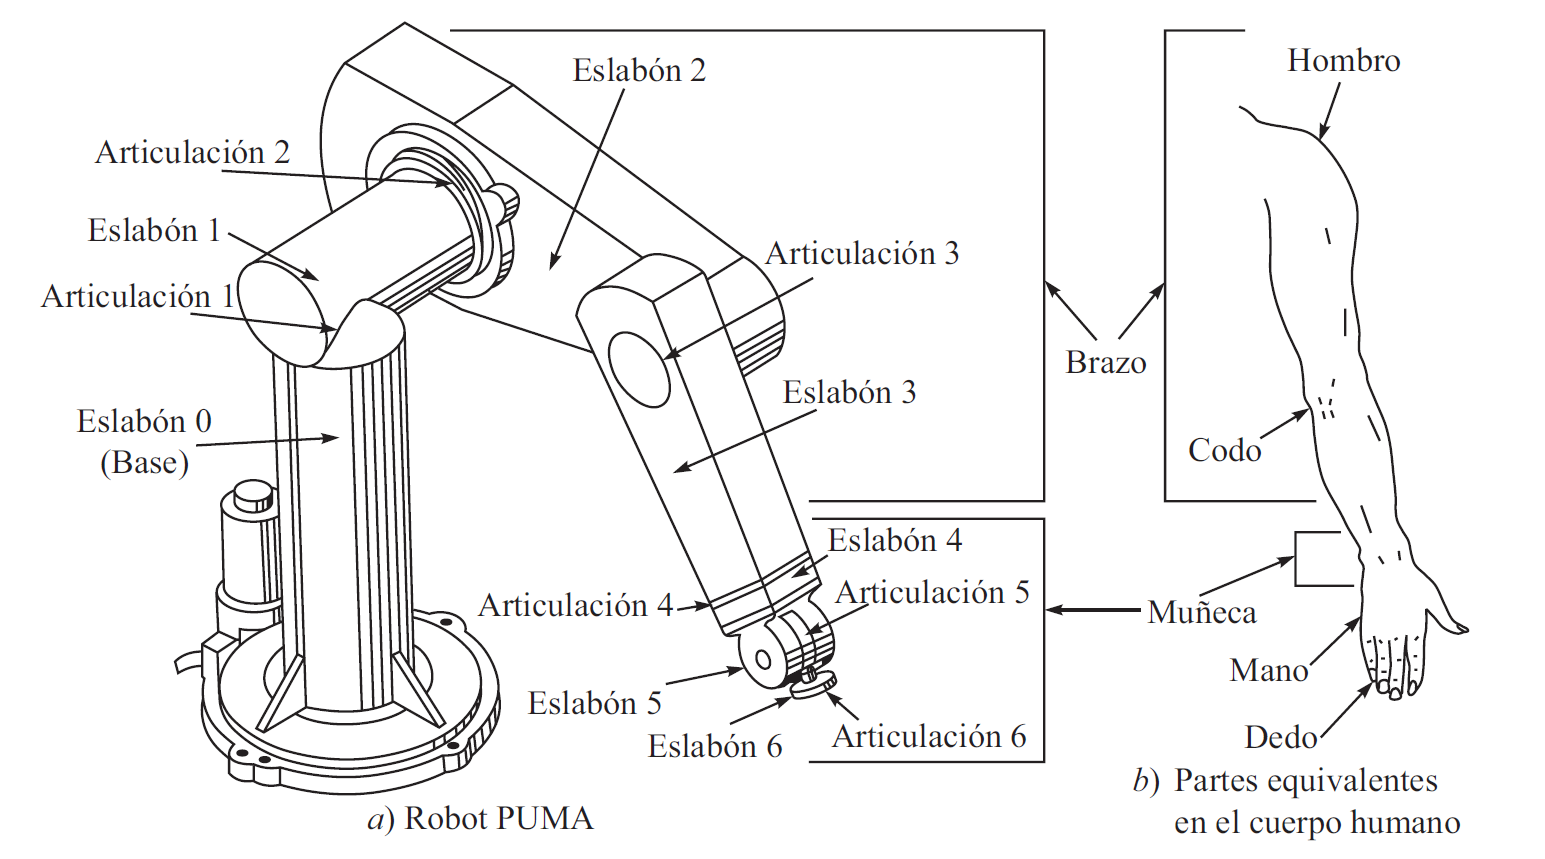
\includegraphics[scale=0.5]{Capitulo1/figs/EstructuraManipulador.png} 
	\caption{Manipulador robótico y sus partes equivalentes en el cuerpo humano}
	\label{estructurarobot}
\end{figure}



%%%%%%%%%%%%%%%%%%%%%%%%%%%%%%%%%%%%%%%%%%%%%%%%%%%%%%%%%%%%%%%%%%%%%%%%%
%                           Objetivo                                    %
%%%%%%%%%%%%%%%%%%%%%%%%%%%%%%%%%%%%%%%%%%%%%%%%%%%%%%%%%%%%%%%%%%%%%%%%%

\subsection{Objetivo}

Diseño y manufactura de un robot manipulador con 5 grados de libertad capaz de realizar seguimiento de trayectorias.
%%%%%%%%%%%%%%%%%%%%%%%%%%%%%%%%%%%%%%%%%%%%%%%%%%%%%%%%%%%%%%%%%%%%%%%%%
%                           Motivación y estado del arte                %
%%%%%%%%%%%%%%%%%%%%%%%%%%%%%%%%%%%%%%%%%%%%%%%%%%%%%%%%%%%%%%%%%%%%%%%%%
\subsection{Motivación}

Los robots manipuladores tienen un amplio uso en la industria y en áreas donde se pretende replicar el trabajo que realiza una persona, ya sea porque es demasiado complejo o se trata de procesos donde se requiera una gran precisión, por encontrarse en ambientes peligrosos o tóxicos, etc. Sin embargo, los robots manipuladores también pueden ser de gran utilidad en el ámbito educativo. Los estudiantes de robótica suelen tener acceso nulo o restringido a manipuladores ya sea por su delicadeza o por la intención de no dañar al robot debido a los elevados costos de reparación. La creación de un manipulador con 5 grados de libertad a un bajo costo pondrá al alcance de los estudiantes una herramienta práctica en el área de la robótica industrial.
%%%%%%%%%%%%%%%%%%%%%%%%%%%%%%%%%%%%%%%%%%%%%%%%%%%%%%%%%%%%%%%%%%%%%%%%%
%                   Planteamiento del problema                          %
%%%%%%%%%%%%%%%%%%%%%%%%%%%%%%%%%%%%%%%%%%%%%%%%%%%%%%%%%%%%%%%%%%%%%%%%%

\subsection{Planteamiento del problema}

El diseño de robots manipuladores es una temática ampliamente abarcada en los trabajos escolares de nivel licenciatura, aunque la mayor parte de esa literatura tiene por objetivo demostrar conceptualmente las capacidades de los robots manipuladores. La construcción del prototipo funcional es un elemento que no se suele llevar a término.
%%%%%%%%%%%%%%%%%%%%%%%%%%%%%%%%%%%%%%%%%%%%%%%%%%%%%%%%%%%%%%%%%%%%%%%%%
%                           Metodología                                 %
%%%%%%%%%%%%%%%%%%%%%%%%%%%%%%%%%%%%%%%%%%%%%%%%%%%%%%%%%%%%%%%%%%%%%%%%%
\subsection{Metodología}

El proceso de construcción del manipulador comienza con el diseño, para ello se plantean los requerimientos y se traducen a especificaciones del robot. Posteriormente se elabora un diseño asistido por computadora donde se obtiene la geometría y espacio de trabajo del manipulador. Se realiza la descripción analítica del movimiento mediante la cinemática directa e inversa, y se termina con la construcción de las piezas y el ensamble del prototipo.

%%%%%%%%%%%%%%%%%%%%%%%%%%%%%%%%%%%%%%%%%%%%%%%%%%%%%%%%%%%%%%%%%%%%%%%%%
%                         Contribuciones                                %
%%%%%%%%%%%%%%%%%%%%%%%%%%%%%%%%%%%%%%%%%%%%%%%%%%%%%%%%%%%%%%%%%%%%%%%%%

\subsection{Contribuciones}

La principal contribución de este trabajo es la simplificación del proceso de construcción para un robot manipulador con 5 grados de libertad, con los elementos necesarios para ser replicado en posteriores trabajos y reduciendo los costos asociados a la fabricación.

%%%%%%%%%%%%%%%%%%%%%%%%%%%%%%%%%%%%%%%%%%%%%%%%%%%%%%%%%%%%%%%%%%%%%%%%%
%                           Estructura de la tesis                      %
%%%%%%%%%%%%%%%%%%%%%%%%%%%%%%%%%%%%%%%%%%%%%%%%%%%%%%%%%%%%%%%%%%%%%%%%%

\subsection{Estructura de la tesis}

En este capítulo se hace una breve descripción del trabajo a desarrollar, el objetivo y algunas ideas generales de robots manipuladores, en el siguiente capítulo se encuentran los fundamentos teóricos que sirven para entender las generalidades de los manipuladores, su composición y la forma de operarlos. En el tercer capítulo se aborda el diseño mecánico junto con un análisis de los elementos que conforman al manipulador, las geometrías y los espacios de trabajo que definirán la movilidad. En el capítulo cuatro se lleva a cabo la construcción del prototipo y la puesta en marcha. En el quinto capítulo se analizan los resultados obtenidos donde se observa la capacidad real del robot manipulador construido y en el último capítulo se tratan las conclusiones y el posible trabajo a futuro del proyecto.

\section{Marco teórico}

Los robots actuales tienen sus orígenes en máquinas controladas remotamente por un operador (teleoperadores) y por máquinas-herramienta controladas numéricamente. A pesar de que el primer teleoperador fue desarrollado en 1947 no fue hasta la década de los 60's cuando los robots manipuladores se incrustaron con éxito en la industria, debido a su alta confiabilidad, repetibilidad y capacidad de adaptación a numerosas actividades. Debajo se encuentra una lista con acontecimientos importantes en el desarrollo de robots manipuladores desde sus inicios al presente.\\\\
1947 - Desarrollo del primer teleoperador servo-eléctrico. El esclavo era servo-controlado para seguir la trayectoria del maestro, sin realimentación.\\\\
1948 - Introducción de un sistema de realimentación en el que la fuerza ejercida por el esclavo era transmitida de vuelta al operador.\\\\
1949 - La Fuerza Aérea de los Estados Unidos patrocinó investigaciones en el desarrollo de herramientas controladas numéricamente. La investigación se realizó para combinar la experiencia en servo-sistemas sofisticados con las recién desarrolladas técnicas de computación digital.\\\\
1954 - George Devol registra una patente en transferencia programada de artículos, Fig (\ref{unimation}).\\\\
1961 - Desarrollo del primer brazo teleoperado equipado con sensores de contacto para dar realimentación de fuerza al operador.\\\\
\begin{figure}[h!]
	\centering
	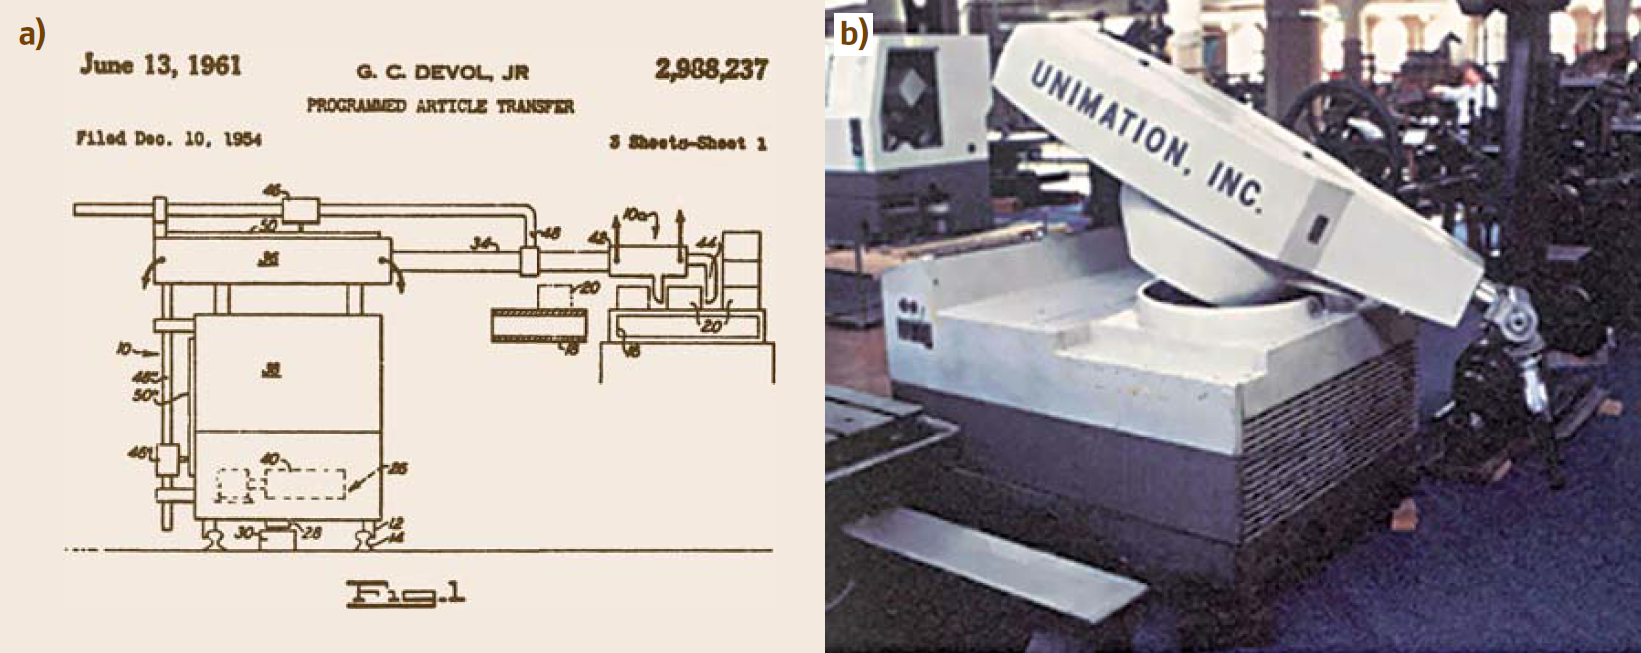
\includegraphics[scale=0.4]{Capitulo1/figs/Unimation.PNG} 
	\caption{(a) La patente de G. Devol marcó el comienzo del trabajo en conjunto con J. Engelberer para crear la primera compañía de robótica del mundo (b) El primer robot instalado en una planta de \textit{General Motors}.}
	\label{unimation}
\end{figure}\\
1963 - Lawrence G. Roberts demuestra la factibilidad de integrar sistemas de visión en los robots.\\\\
1969 - Victor Scheinman diseña \textit{The Stanford Arm}, uno de los primeros manipuladores en ser concebidos exclusivamente para control por computadora. Fig(\ref{stfarm})\\
\begin{figure}[h!]
	\centering
	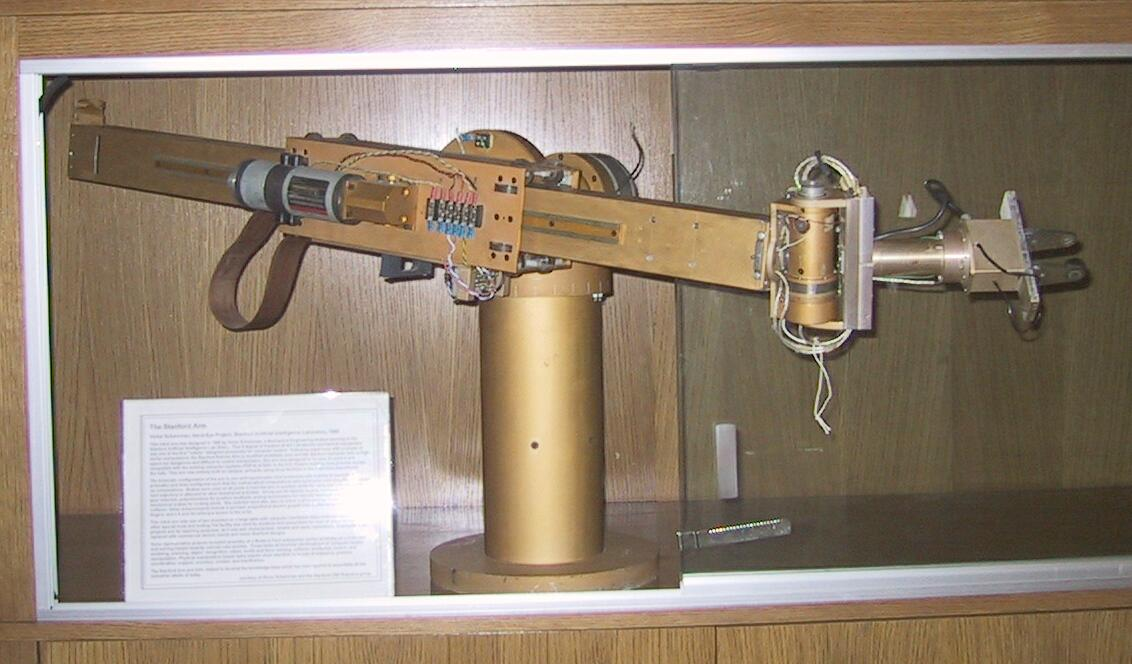
\includegraphics[scale=0.3]{Capitulo1/figs/StanfordArm.jpg} 
	\caption{\textit{The Stanford Arm}. La configuración no es antropomórfica, cuenta con 6 pares cinemáticos (5 rotacionales, 1 prismático).}
	\label{stfarm}
\end{figure}\\
1973 - Creación del primer lenguaje de programación para robots \textit{WAVE} en la Universidad de Stanford.\\\\
1974 - La compañía Cincinnati Milacron introduce el robot T3 con control por computadora integrado.\\\\
1976 - Avión\\\\
            % ~10 páginas - Explicar el propósito de la tesis

%%%%%%%%%%%%%%%%%%%%%%%%%%%%%%%%%%%%%%%%%%%%%%%%%%%%%%%%%%%%%%%%%%%%%%%%%
%       Capítulo 2: Descripción de un robot de 5 grados de libertad     %
%%%%%%%%%%%%%%%%%%%%%%%%%%%%%%%%%%%%%%%%%%%%%%%%%%%%%%%%%%%%%%%%%%%%%%%%%

\chapter{\textcolor{Azul}{Descripción de un robot de 5 grados de libertad}}

\section{Articulaciones y pares cinemáticos}

La movilidad de un sistema puede expresarse en función de los parámetros independientes mínimos que se necesitan para describir de manera única su posición y orientación en un instante de tiempo [6]. Estos parámetros reciben por nombre \textbf{grados de libertad} (GDL). El número de GDL también depende de las dimensiones del espacio en el que se trabaje. Para ejemplificar el caso del movimiento en un espacio plano de dos dimensiones se puede tomar un cuadrado de papel y colocarlo sobre un escritorio, el papel puede moverse de manera vertical (primer GDL), horizontal (segundo GDL) o girar sobre un eje perpendicular al plano (tercer GDL). Dichos movimientos también pueden limitarse. Si ahora se toma un alfiler y se clava el cuadrado de papel sobre el escritorio se han restringido los movimientos horizontales y verticales, quedando únicamente la rotación alrededor del alfiler (solamente un GDL).\\\\En el caso del movimiento plano, los cuerpos rígidos sin restricción cuentan con tres GDL, dos que indican posición y uno que indica orientación. Si se considera ahora el espacio tridimensional, los cuerpos rígidos cuentan con seis GDL, se necesitan tres para definir la posición y otros tres que definen la orientación. \\

\\Los eslabones que componen a un robot manipulador están conectados de tal manera que se permita cierto tipo de movimiento. Existen dos movimientos a partir de los cuales se derivan cualquier movimiento complejo conocido: la traslación pura y la rotación pura. Estas conexiones entre eslabones reciben el nombre de articulaciones o pares cinemáticos [7], Fig \ref{pares}.

\begin{figure}
	\centering
	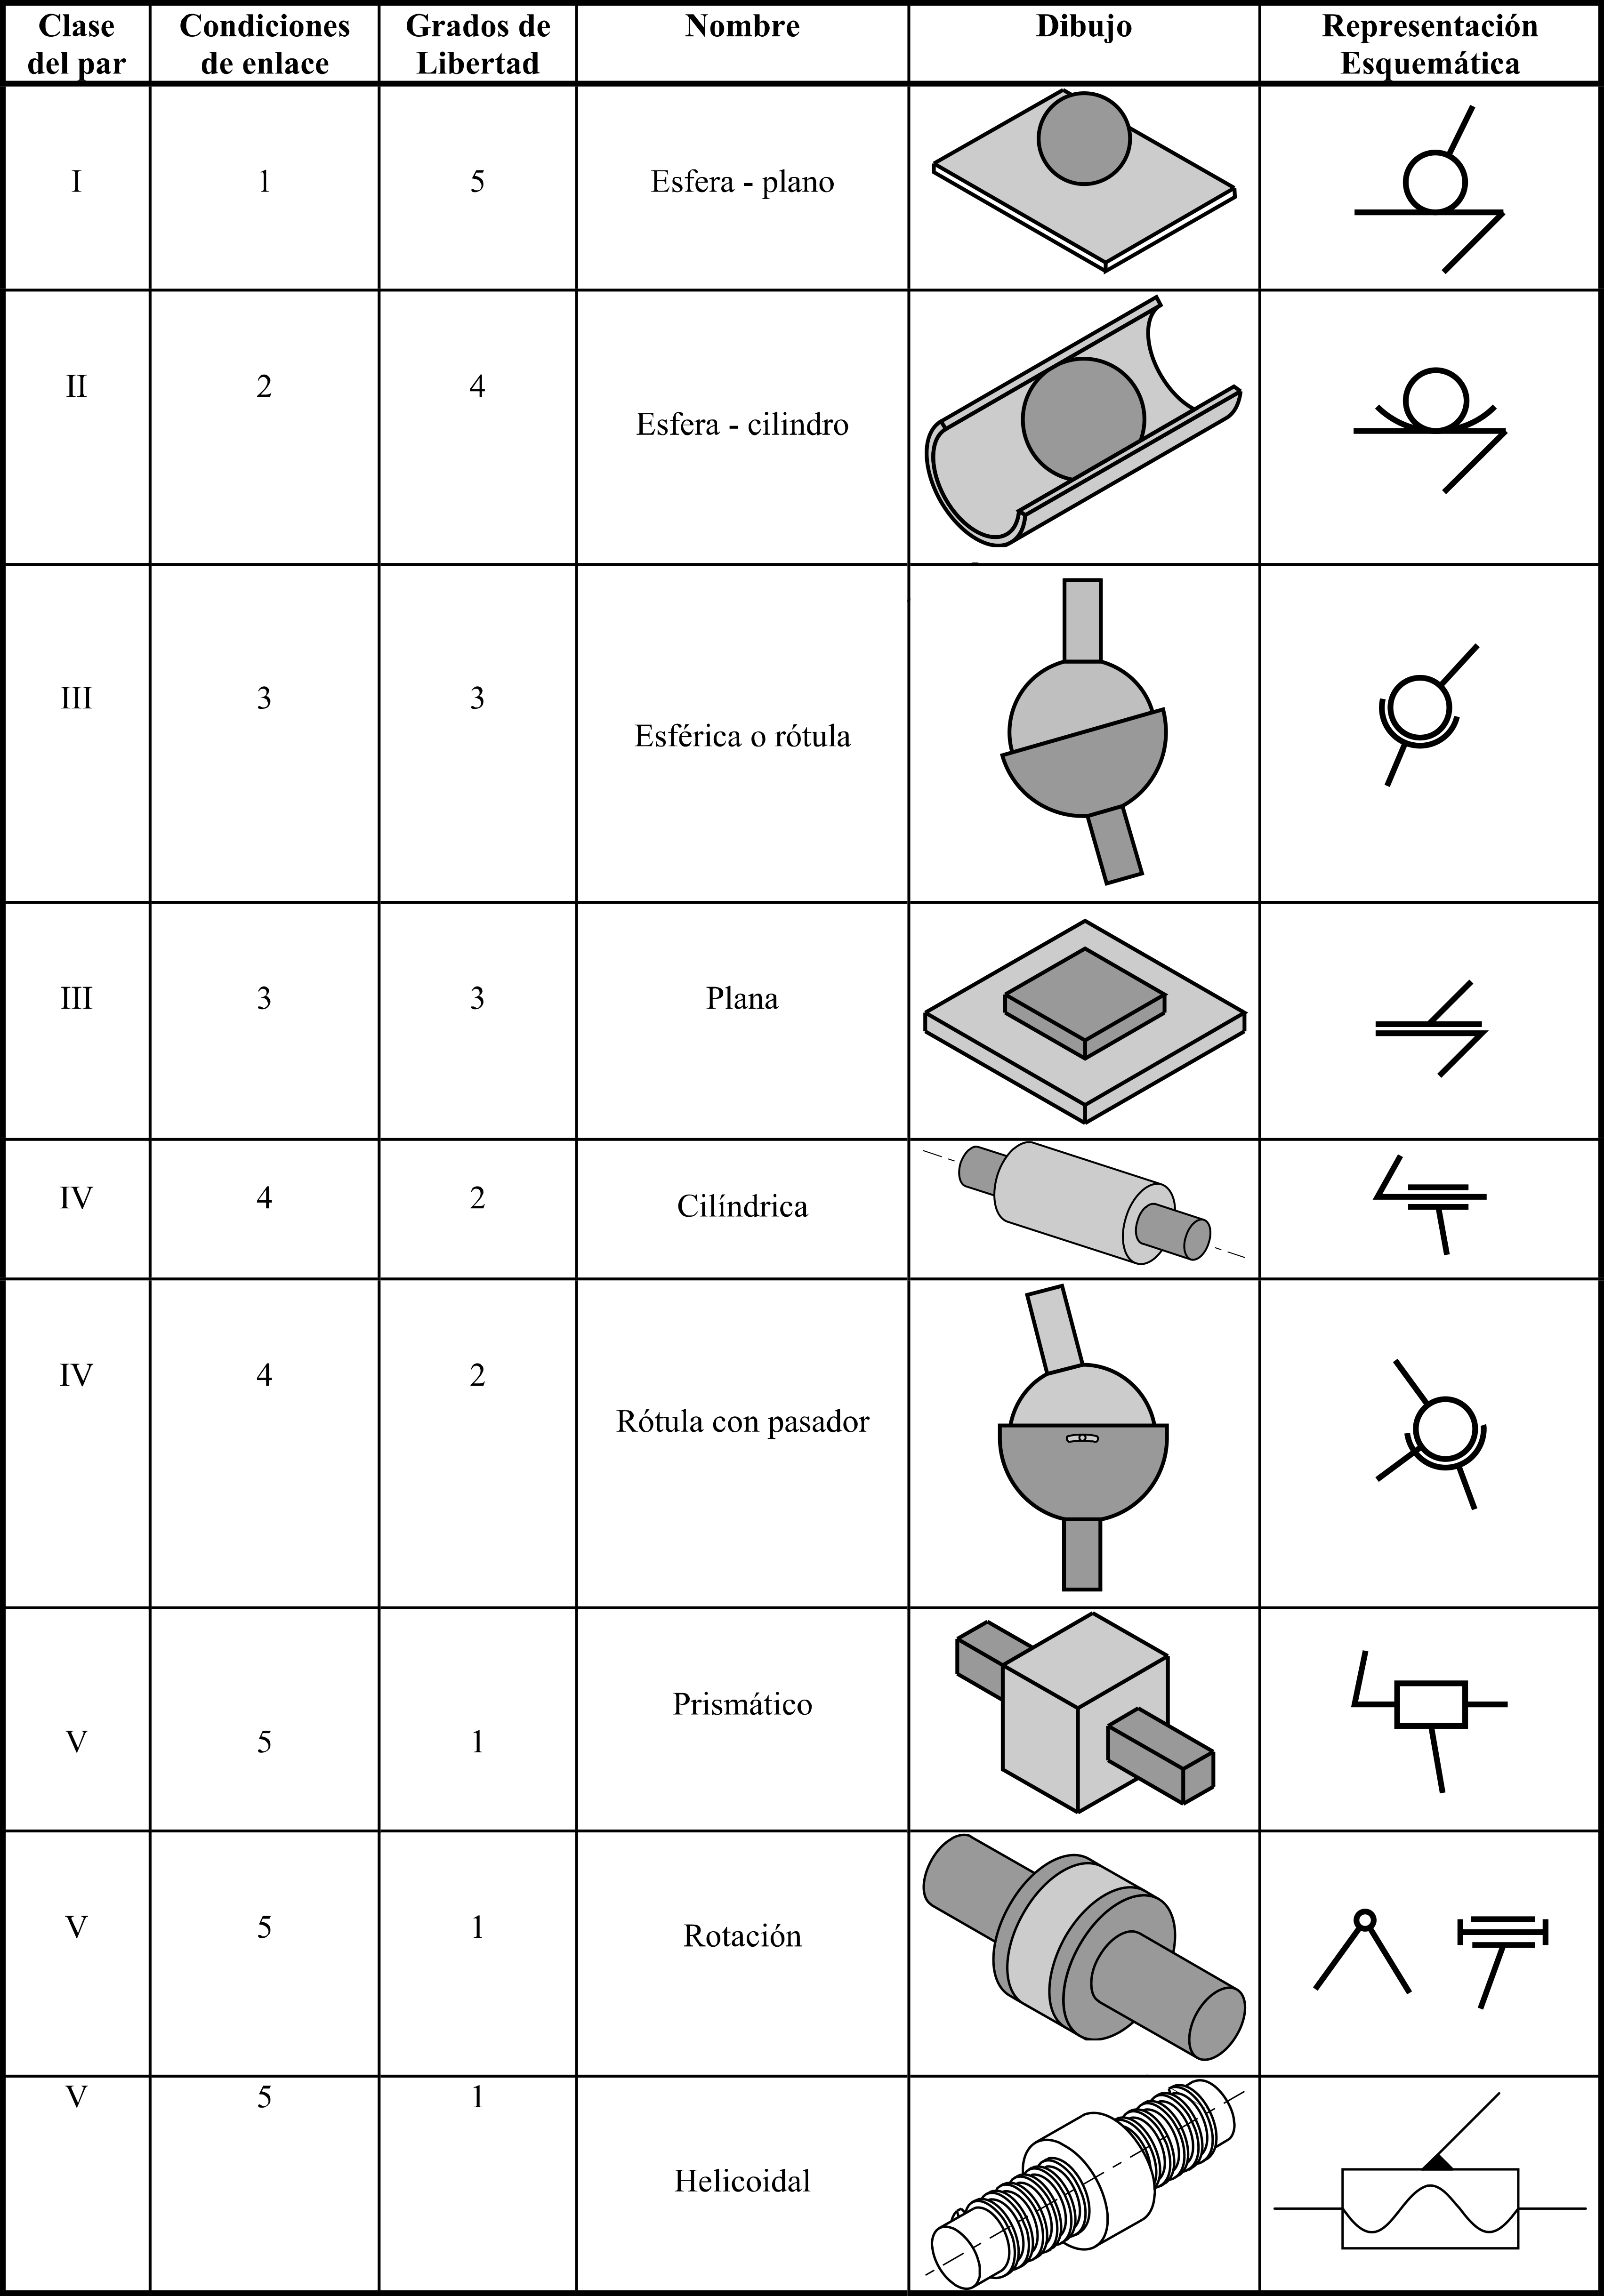
\includegraphics[scale=1.0]{Capitulo2/figs/pares.png} 
	\caption{Pares cinemáticos superiores e inferiores}
	\label{pares}
\end{figure}

\section{Cinemática directa}

Los robots rígidos guardan una relación entre la posición individual de cada articulación y la ubicación espacial de la herramienta o efector final. Una gran parte de la cinemática de los robots se encarga de establecer sistemas de coordenadas para cada eslabón rígido, indicando la posición y orientación respecto a un sistema de referencia inercial, que se relacionan entre sí mediante matrices de transformación. Las operaciones básicas entre sistemas de coordenadas son la traslación y la rotación, que pueden combinarse para obtener matrices de transformaciones homogéneas, como se describirá más adelante. \\\\


\subsection{Posición}



\subsection{Orientación}

\section{Cinemática inversa}

\section{Modelado}

%inserción de codigo de Matlab
%Es conveniente sangrarlo (los de proteco dicen "indentarlo") para que no se encime con los números de las líneas a la izquierda
\begin{lstlisting}[frame=single]
    % Declaracion de las variables simbolicas
\end{lstlisting}           % ~20 páginas - Poner un contexto a la tesis, hacer referencia a trabajos actuales en el tema

%%%%%%%%%%%%%%%%%%%%%%%%%%%%%%%%%%%%%%%%%%%%%%%%%%%%%%%%%%%%%%%%%%%%%%%%%
%           Capítulo 3: Control               %
%%%%%%%%%%%%%%%%%%%%%%%%%%%%%%%%%%%%%%%%%%%%%%%%%%%%%%%%%%%%%%%%%%%%%%%%%

\chapter{\textcolor{Azul}{Control}}
En este capítulo, se presenta la introducción al desarrollo de la tesis, ya sea el modelo matemático o las bases del proyecto, etc.
%Ejemplo de cita  [\citet{latex}]
%Ejemplo de cita [\citeauthor{RR73}]
 % The \cite command functions as follows:
 %   \citet{key} ==>>                Jones et al. (1990)
 %   \citet*{key} ==>>               Jones, Baker, and Smith (1990)
 %   \citep{key} ==>>                (Jones et al., 1990)
 %   \citep*{key} ==>>               (Jones, Baker, and Smith, 1990)
 %   \citep[chap. 2]{key} ==>>       (Jones et al., 1990, chap. 2)
 %   \citep[e.g.][]{key} ==>>        (e.g. Jones et al., 1990)
 %   \citep[e.g.][p. 32]{key} ==>>   (e.g. Jones et al., p. 32)
 %   \citeauthor{key} ==>>           Jones et al.
 %   \citeauthor*{key} ==>>          Jones, Baker, and Smith
 %   \citeyear{key} ==>>             1990

%%%%%%%%%%%%%%%%%%%%%%%%%%%%%%%%%%%%%%%%%%%%%%%%%%%%%%%%%%%%%%%%%%%%%%%%%
%                          Descripción de la planta                     %
%%%%%%%%%%%%%%%%%%%%%%%%%%%%%%%%%%%%%%%%%%%%%%%%%%%%%%%%%%%%%%%%%%%%%%%%%
\section{Conceptos de control}

A pesar de la existencia de robots comerciales de tipo industrial, diseñar controladores para robots sigue siendo un área compleja y constantemente estudiada por parte de los constructores de robots, así como por centros de investigación en control y robótica alrededor del mundo. Podría argumentarse que los robots industriales actuales son capaces de realizar correctamente una gran variedad de tareas, por lo que pareciera innecesario el desarrollo de investigaciones sobre el tema de control de robots. Sin embargo, este último tema, además de interesante, tiene muchos retos que ofrecer en el marco teórico, y más importante aún, su estudio es indispensable en aplicaciones específicas que no pueden ser llevadas a cabo mediante los robots comerciales actuales.\\

La metodología de diseño de los sistemas de control puede resumirse en los siguientes pasos:

\begin{itemize}
	\item Familiarización con el sistema físico a controlarse.
	\item Modelado.
	\item Especificaciones de control.
\end{itemize}

\subsection{Familiarización con el sistema fisico a controlarse}

En esta primera etapa deben identificarse las \textit{salidas del sistema}, que son todas aquellas variables físicas que se desea gobernar, tales como velocidad, desplazamiento, temperatura, etc. Además deben identificarse claramente aquellas variables físicas del sistema que se encuentran disponibles y que influyen en el comportamiento del mismo, y en particular afectan a las salidas del sistema. Estas variables llamadas \textit{entradas del sistema} pueden ser, por ejemplo, corriente eléctrica, par o fuerza, tensión, etc.\\

En el caso de los robots manipuladores, la variable de salida (denotada momentaneamente por \textbf{y}) cuya conducta se desea modificar, ofrece un amplio espectro de elecciones tal como podemos ver a continuación.\\

\subsection{Modelado dinámico}


\subsection{Especificaciones de control}

%Ejemplo de cita \citep{texbook}


%%%%%%%%%%%%%%%%%%%%%%%%%%%%%%%%%%%%%%%%%%%%%%%%%%%%%%%%%%%%%%%%%%%%%%%%%
%                          Modelado                                     %
%%%%%%%%%%%%%%%%%%%%%%%%%%%%%%%%%%%%%%%%%%%%%%%%%%%%%%%%%%%%%%%%%%%%%%%%%
\section{Esquemas de control}

\subsection{PID}

\section{Control por par calculado}

\section{Parámetros de diseño}
Antes de comenzar, se definen  en la tabla ~\ref{tab:tabla} los parámetros y variables utilizadas

%%%%%%%%Tabla Nombres de parámetros
\begin{table}[htdp]                             %Inicia el entorno table debajo del texto
\centering\                                     %   centra la tabla
\begin{tabular}{||c | c ||}                     %inicia entorno tabular con doble línea en las orillas, 2 columnas con el contenido centrado (c)
\hline                                          %inserta línea horizontal
\hline
Nombre Parámetro/Variable & Símbolo\\
\hline
\hline
Masa del péndulo & $m$ \\
\hline
Masa del carro & $M$\\
\hline
Distancia del eje de giro al centro de masa & $l$ \\
\hline
Aceleración gravitatoria & $g$ \\
\hline
Momento de inercia péndulo respecto del eje de giro& $J$ \\
\hline
Ángulo del péndulo respecto del eje vertical & $\theta$\\
\hline
Velocidad angular del péndulo & $\dot{\theta}$, $\omega$\\
\hline
Distancia del carro respecto al centro del riel & x\\
\hline
Velocidad del carro & $\dot{x}$, $v$\\
\hline
\hline
\end{tabular}
\caption[Tabla 1]{\textbf{Parámetros dinámicos del carro-péndulo} - Estos son los valores de parámetros utilizados en el diseño y las simulaciones, corresponden a los valores reales.}
\label{tab:tabla}                              %etiqueta para referencia
\end{table}
      % ~20 páginas - Explicar el problema en específico que se va a resolver, la metodología y experimentos/métodos utilizados

%%%%%%%%%%%%%%%%%%%%%%%%%%%%%%%%%%%%%%%%%%%%%%%%%%%%%%%%%%%%%%%%%%%%%%%%%
%                    Capítulo 4: Diseño Mecánico                       %
%%%%%%%%%%%%%%%%%%%%%%%%%%%%%%%%%%%%%%%%%%%%%%%%%%%%%%%%%%%%%%%%%%%%%%%%%

\chapter{\textcolor{Azul}{Diseño Mecánico}}

\section{Elementos físicos}

\section{Barras, rodamientos, contrapesos}

\section{Métodos de unión}
   % ~20 páginas - Presentar los resultados tal cual son, y analizarlos.

%%%%%%%%%%%%%%%%%%%%%%%%%%%%%%%%%%%%%%%%%%%%%%%%%%%%%%%%%%%%%%%%%%%%%%%%%
                   % Capítulo 5: Manufactura e instrumentación          %
%%%%%%%%%%%%%%%%%%%%%%%%%%%%%%%%%%%%%%%%%%%%%%%%%%%%%%%%%%%%%%%%%%%%%%%%%


\chapter{\textcolor{Azul}{Manufactura e instrumentación}}

La figura (\ref{gripper01})                     %hace referencia a la imagen "planta" el número se inserta automáticamente
ilustra la geometría del efector final

\begin{figure}
	\centering
	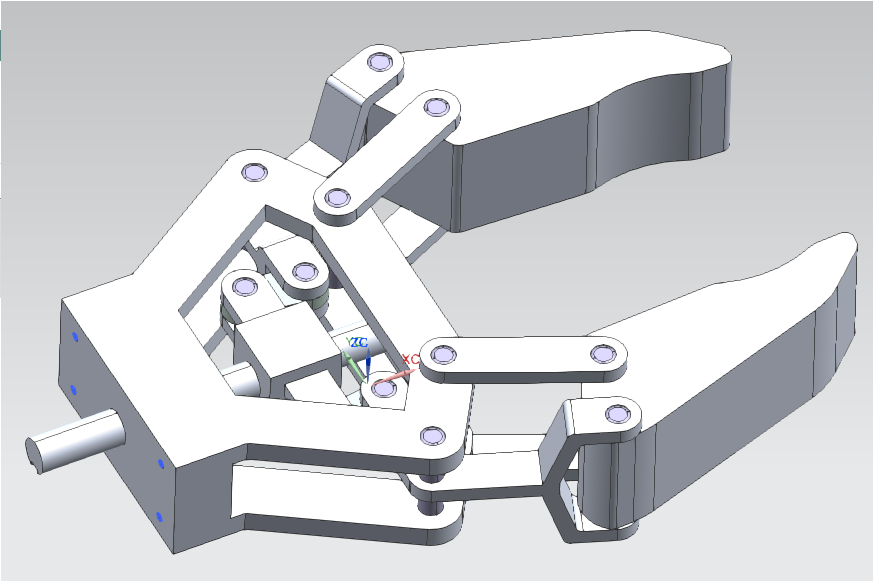
\includegraphics[scale=0.5]{Capitulo5/figs/Gripper.png}      %Ruta completa de la imagen, porque se compila desde el archivo tesis.tex
	\caption{Órgano Terminal}            %Pie de imagen
	\label{gripper01}                            %nombre de referencia
\end{figure}


\section{Ensamble de componentes}

\section{Sensores y actuadores}

\subsection{Motores}

\subsection{Decodificador óptico}

Para obtener datos que representen la posición y orientación de los eslabones se utiliza un deco

\section{Microcontrolador}            % ~5 páginas - Resumir lo que se hizo y lo que no y comentar trabajos futuros sobre el tema

%%%%%%%%%%%%%%%%%%%%%%%%%%%%%%%%%%%%%%%%%%%%%%%%%%%%%%%%%%%%%%%%%%%%%%%%%
%                Capítulo 6: Implementación                            %
%%%%%%%%%%%%%%%%%%%%%%%%%%%%%%%%%%%%%%%%%%%%%%%%%%%%%%%%%%%%%%%%%%%%%%%%%

\chapter{\textcolor{Azul}{Implementación}}

\section{Programación}

\section{Puesta en marcha}

\section{Pruebas mecánicas}
%%%%%%%%%%%%%%%%%%%%%%%%%%%%%%%%%%%%%%%%%%%%%%%%%%%%%
%                   APÉNDICES                       %
%%%%%%%%%%%%%%%%%%%%%%%%%%%%%%%%%%%%%%%%%%%%%%%%%%%%%
\appendix

%%%%%%%%%%%%%%%%%%%%%%%%%%%%%%%%%%%%%%%%%%%%%%%%%%%%%%%%%%%%%%%%%%%%%%%%%
%                          Resultados                                   %
%%%%%%%%%%%%%%%%%%%%%%%%%%%%%%%%%%%%%%%%%%%%%%%%%%%%%%%%%%%%%%%%%%%%%%%%%

\chapter{Resultados}

% this file is called up by thesis.tex
% content in this file will be fed into the main document
\chapter{Referencias}
% top level followed by section, subsection

[1] Karel Capek. (1920). R. U. R.(Rossum's Universal Robots).

[2] Real Academia Española. (2017). Diccionario de la lengua española (23.a ed.). Consultado en http://www.rae.es/rae.html

[3] Mark W. Spong, Seth Hutchinson, M. Vidyasagar. (2004). Robot Dynamics and Control. Lugar de publicación. Editorial.

\chapter{Conclusiones/Trabajo a futuro}

Apéndice
               % Colocar los circuitos, manuales, código fuente, pruebas de teoremas, etc.

%%%%%%%%%%%%%%%%%%%%%%%%%%%%%%%%%%%%%%%%%%%%%%%%%%%%%
%                   REFERENCIAS                     %
%%%%%%%%%%%%%%%%%%%%%%%%%%%%%%%%%%%%%%%%%%%%%%%%%%%%%
% existen varios estilos de bilbiografía, pueden cambiarlos a placer
\bibliographystyle{apalike} % otros estilos pueden ser abbrv, acm, alpha, apalike, ieeetr, plain, siam, unsrt

%El formato trae otros estilos, o pueden agregar uno que les guste:
%\bibliographystyle{Latex/Classes/PhDbiblio-case} % title forced lower case
%\bibliographystyle{Latex/Classes/PhDbiblio-bold} % title as in bibtex but bold
%\bibliographystyle{Latex/Classes/PhDbiblio-url} % bold + www link if provided
%\bibliographystyle{Latex/Classes/jmb} % calls style file jmb.bst

\bibliography{Bibliografia/referencias}             % Archivo .bib


\end{document}